\section{BlkKin Design}

\begin{frame}[t]{Outline}
\setcounter{tocdepth}{1}
\tableofcontents[currentsection]
\end{frame}

\begin{frame}{BlkKin = Block Storage + Zipkin}
BlkKin is:
\hfill \\
\begin{itemize}
\item end-to-end tracing infrastructure
\item implementing Dapper semantics
\item based on Zipkin and LTTng 
\item providing live tracing
\end{itemize}
\end{frame}

\begin{frame}{BlkKin Contribution}
\begin{center}
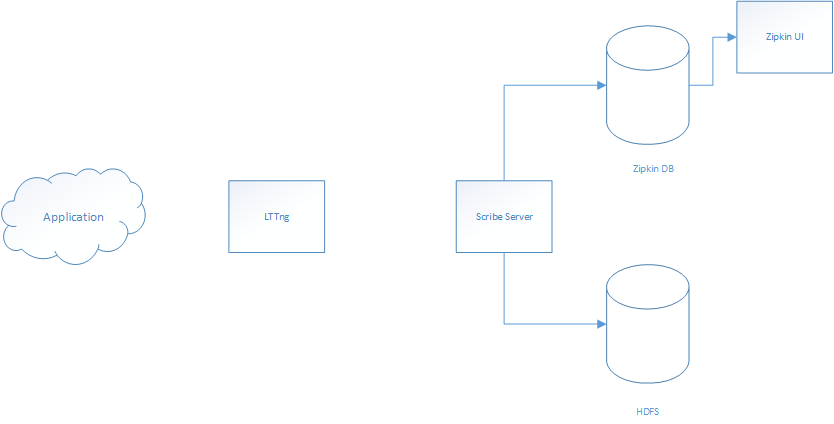
\includegraphics[scale=0.45]{images/step1.png}
\end{center}
\end{frame}

\begin{frame}{BlkKin Contribution}
\begin{center}
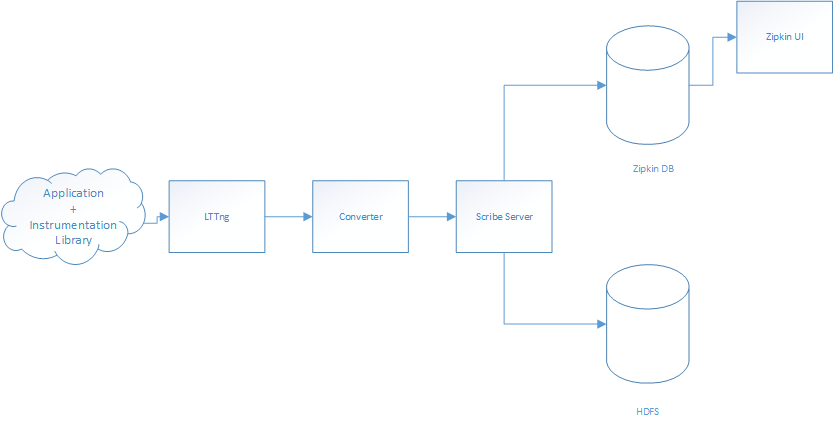
\includegraphics[scale=0.45]{images/step2.png}
\end{center}
\end{frame}

\begin{frame}{BlkKin Contribution}
\begin{center}
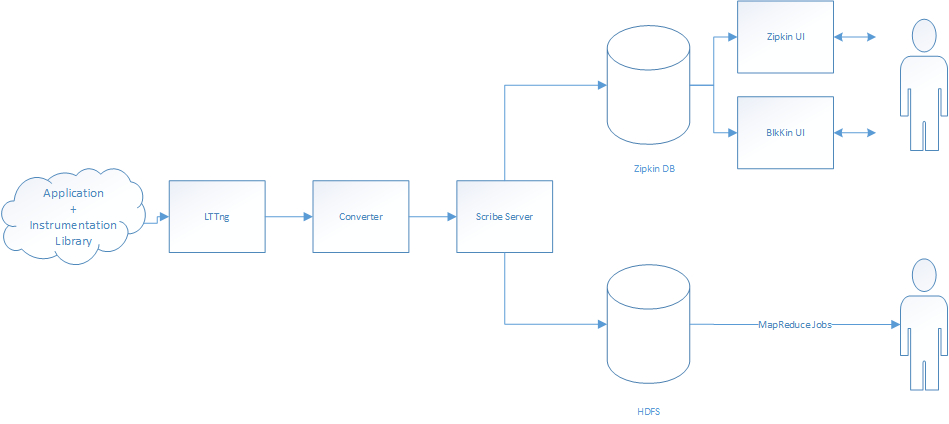
\includegraphics[scale=0.45]{images/step3.png}
\end{center}
\end{frame}

\begin{frame}{BlkKin Contribution}
BlkKin instrumentation library:
\begin{itemize}
\item C/C++ instrumentation library
\item implementing Dapper tracing semantics
\item LTTng backend
\item sampling
\end{itemize}

\hfill \\
CTF-to-Scribe Babeltrace plugins:
\begin{itemize}
\item based on Python bindings
\item two output formats: 
    \begin{itemize}
    \item JSON format (generic)
    \item Zipkin Thrift (Zipkin specific)
    \end{itemize}
\end{itemize}
\end{frame}

\begin{frame}{BlkKin Architecture}
\begin{center}
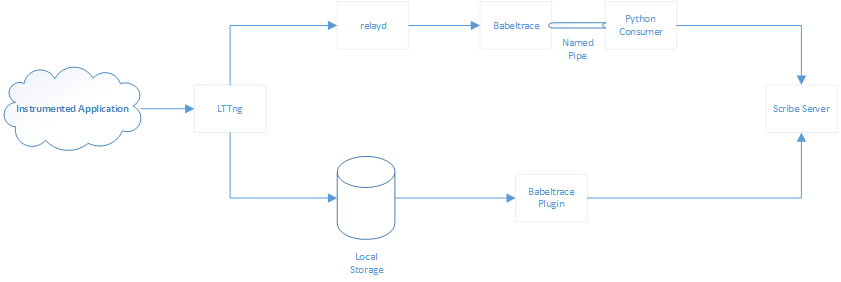
\includegraphics[scale=0.52]{images/blkin-internal.png}
\end{center}
\end{frame}

\begin{frame}{BlkKin Architecture}
\begin{center}
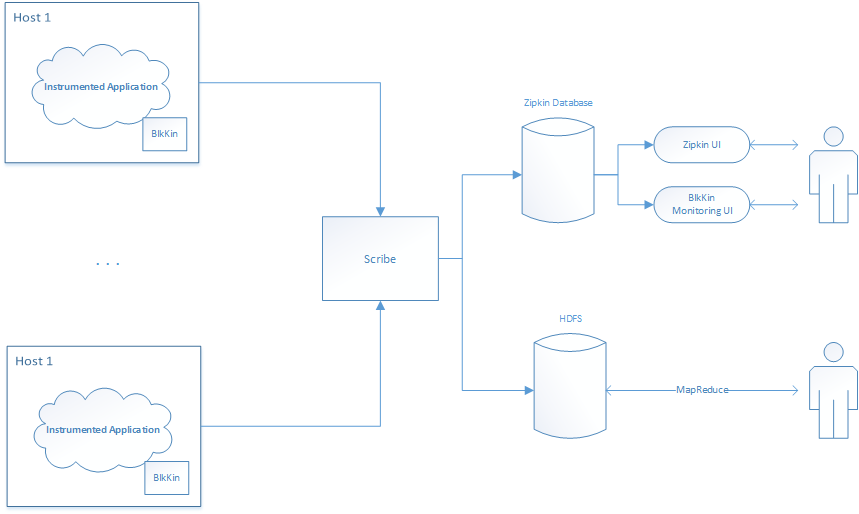
\includegraphics[scale=0.5]{images/blkin-deploy.png}
\end{center}
\end{frame}
